\chapter{Oracle Application Express}
    \section{Pengertian}
        Oracle Application Express (Oracle APEX) adalah sebuah platform yang digunakan untuk pengembangan aplikasi kode rendah. Kode rendah dimaksud disini yaitu mudah di ramp, super produktif, scaleable, extensible, dan fungsionalitas kaya dengan kode yang sedikit. Yang memungkinkan Anda membuat aplikasi perusahaan yang dapat diskalakan dan aman dengan fitur kelas dunia yang bisa digunakan di mana saja. Adapun alat utama yang terdapat pada oracle application express
        \begin{figure}[!htbp]
        \centering
        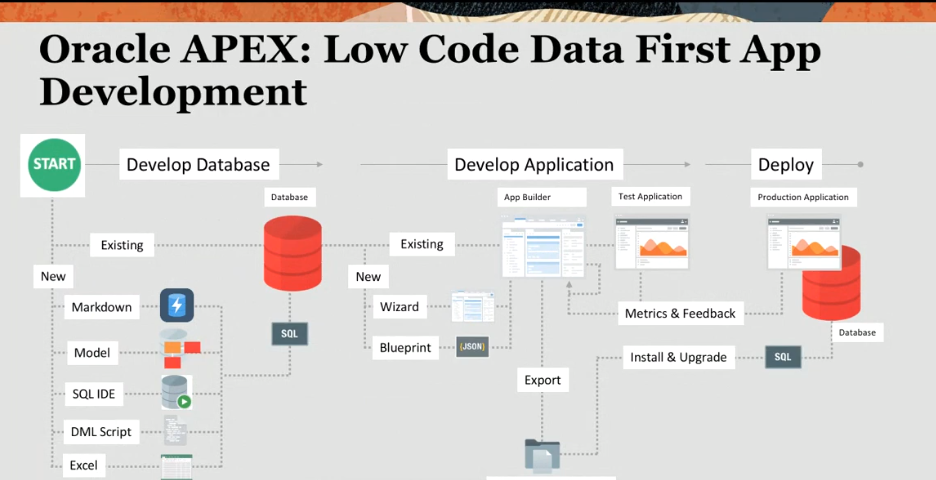
\includegraphics[scale=0.6]{figures/1.PNG}
        \caption{Oracle application express}
    \end{figure}
\begin{enumerate}
    \item Application Builder : Yang digunakan untuk membuat aplikasi, melihat
aplikasi, mengimport aplikasi, mengatur service, mengatur user aplikasi dan
memantau aktifitas yang dilakukan pengguna.
    \item SQL Workshop : Yang digunakan untum membuat table dan komponennya (menggnakan kode PL – SQL secara manual maupun otomatis), melihat
struktur table dan komponennya, mengimpor dan mengekspor script.
    \item Utilitas : Yang digunakan untuk melihat report table dan komponennya serta history aplikasi. kerangka kerja pengembangan aplikasi web database sentris terdiri dari 3 yaitu:
    \begin{enumerate}
        \item mengembangkan aplikasi web desktop dan aplikasi web seluler
        \item memvisualisasikan dan memelihara data database
        \item meningkatkan keterampilan sql dan kemampuan database
    \end{enumerate}
    \item Macam aplikasi oracle yg cocok untuk pengguna
    \begin{enumerate}
        \item Aplikasi yang penting bagi ribuan pengguna
        \item Mengisi kesenjangan dalam sistem perusahaan
        \item Merampingkan proses bisnis yang kadaluarsa
        \item Modernisasi sistem warisan
        \item Aplikasi layanan mandiri untuk semua karyawan
        \item Portal yang menghadap pelanggang / mitra
        \item Aplikasi responsif yang bekerja pada perangkat apapun 
        \item Bukti konsep, aplikasi yang cepat menang, dan menggantikan spreadsheet
    \end{enumerate}
\end{enumerate}
\section{Kekurangan Spreadsheets}
   Menggunakan spreadsheet untuk mengolah data terdapat banyak kekurangan, seperti pada validasi datanya rawan manual dan kesalahan, integritas data tidak dapat menjamin keakuratan data dalam lingkunhgan multi-user, keamanan data penguncian sel tidak efektif, berbagi data pada excel lamban dan sulit di bagikan. Sehingga sekarang digunakan Oracle Application Express untuk menghindari kekurangan-kekurangan saat menggunakan spreadsheet.
\section{Contoh Database Tunggal/Beberapa Workspace}
    Keunggulan dari UI apex ini yaitu mudah diakeses pada perangkat yang sepenuhnya dapat disesuaikan dan responsif aplikasi
    \begin{enumerate}
    \item Ruang kerja yang digunakan untuk mendefinisikan aplikasi / memegang skema data
    \item Banyak ke banyak hubungan antara ruang kerja dan skema
    \item Instance administrator mengelolah lingkungan dan skema akses
    \item Department dapat meminta lebih banyak ruang, dan akses ke skema baru.
    \end{enumerate}
\section{Cara membuat workspace}
\begin{enumerate}
    \item Yang pertama yaitu lakukan instalasi apex pada komputer
    \item Buka link web apex
        \item Kedua, buka link web apex http://127.0.0.1:8080/apex/f?p=4550:10:384005553208::::: 
        Masuk sebagai admin lalu masukkan user dan password yang sudah anda buat. lalu sign in to administration.
    \begin{figure}[!htbp]
        \centering
        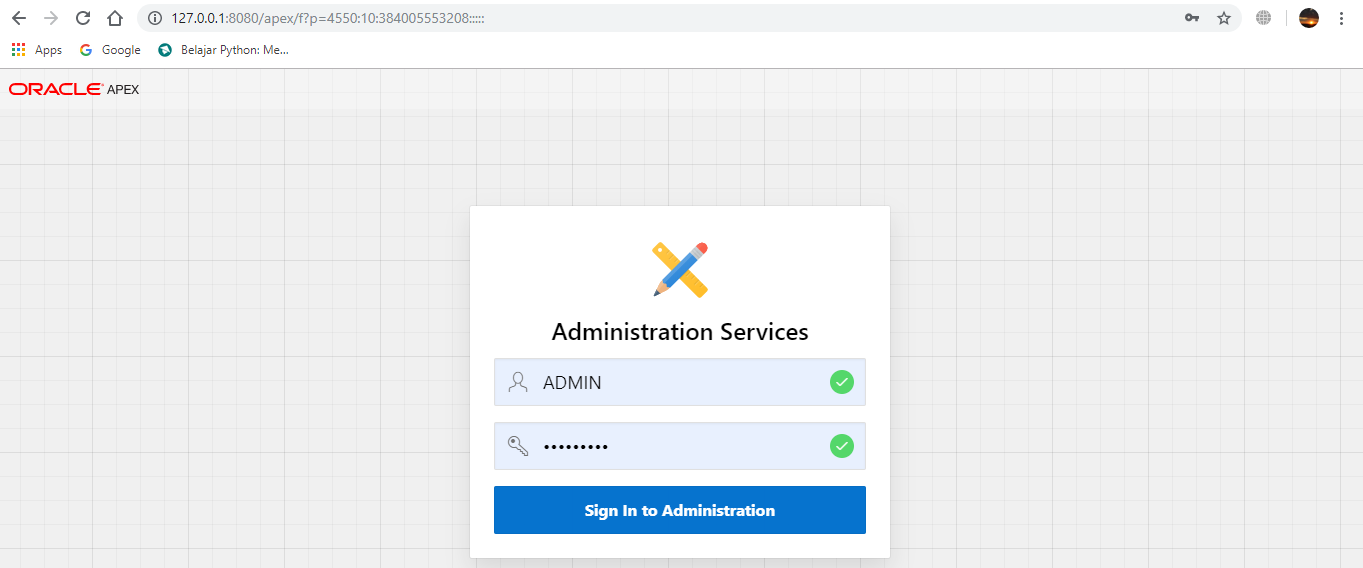
\includegraphics[scale=0.3]{figures/a.PNG}
        \caption{Halaman Utama Apex Sign In}
     \end{figure}
    \item  akan masuk langsung ke halaman utama
     \begin{figure}[!htbp]
        \centering
        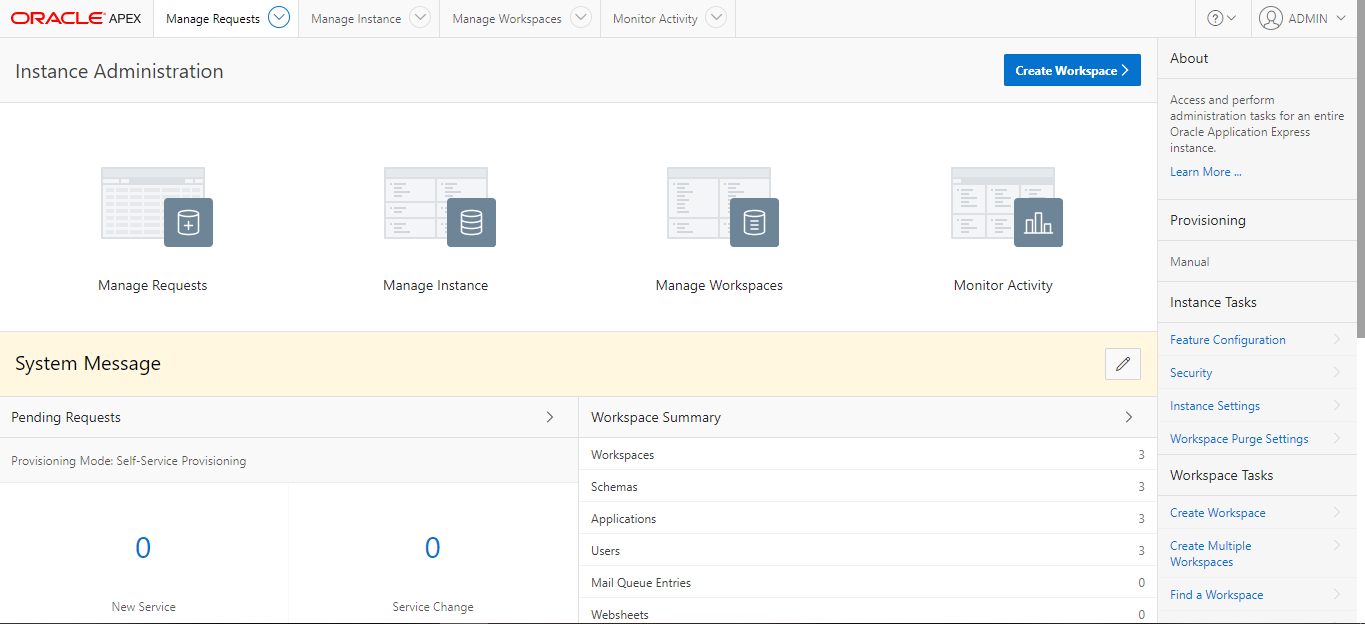
\includegraphics[scale=0.3]{figures/n1.PNG}
        \caption{Login Workspace}
    \end{figure}
    \item Setelah itu klik \textit{Create Workspace}
    \begin{figure}[!htbp]
        \centering
        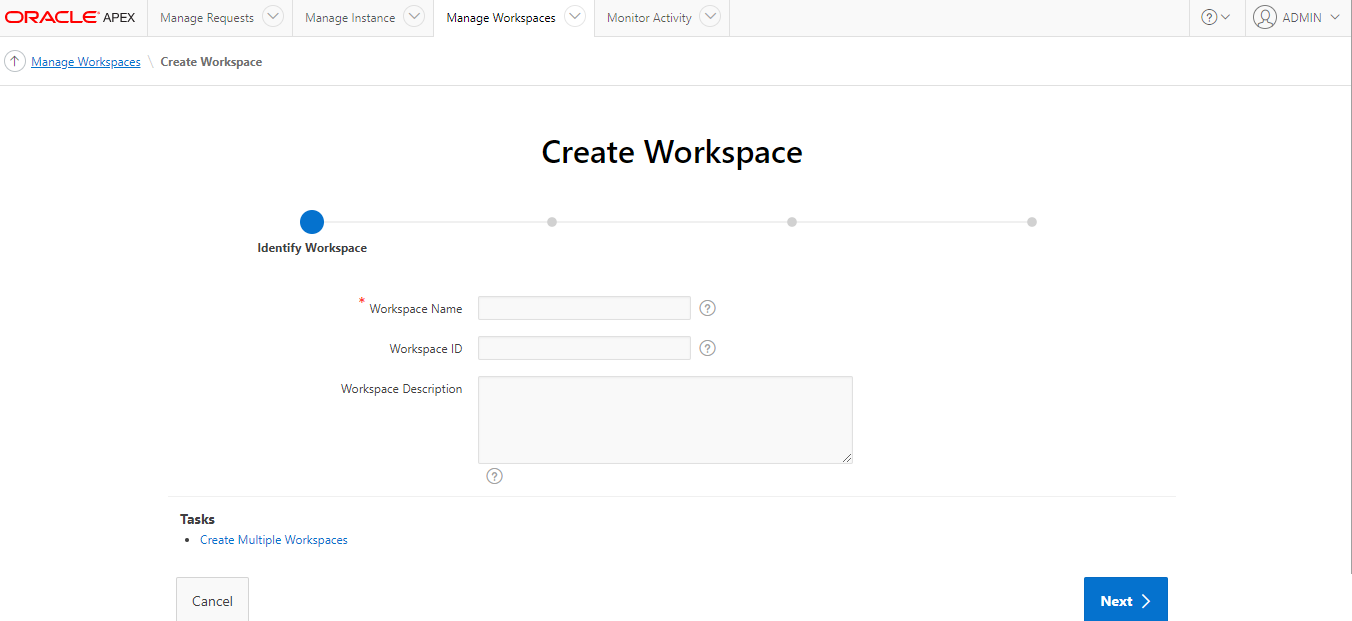
\includegraphics[scale=0.3]{figures/n2.PNG}
        \caption{Create Workspace}
    \end{figure}
\newpage
    \item Isi nama dari workspace yang akan dibuat, selain nama workspace dapat dikosongkan karena tidak berpengaruh.
    \begin{figure}[!htbp]
        \centering
        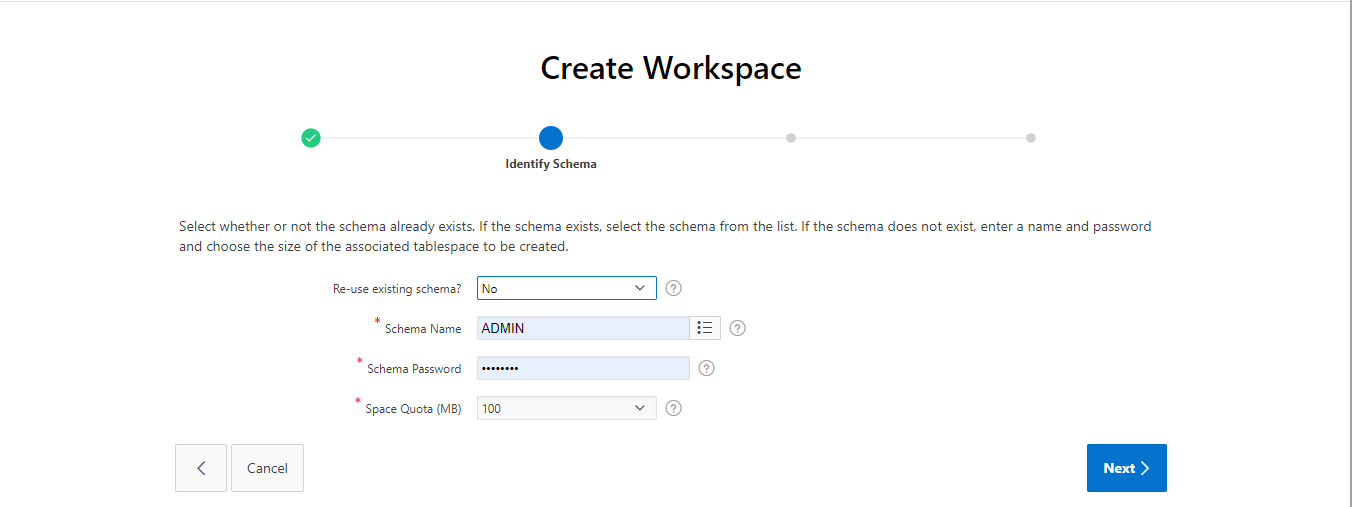
\includegraphics[scale=0.3]{figures/n3.PNG}
        \caption{Pemberian Nama Pada Workspace}
    \end{figure}
    \item Setelah itu, klik next
    \item Buatlah pengaturan sebagai berikut.
    \begin{figure}[!htbp]
        \centering
        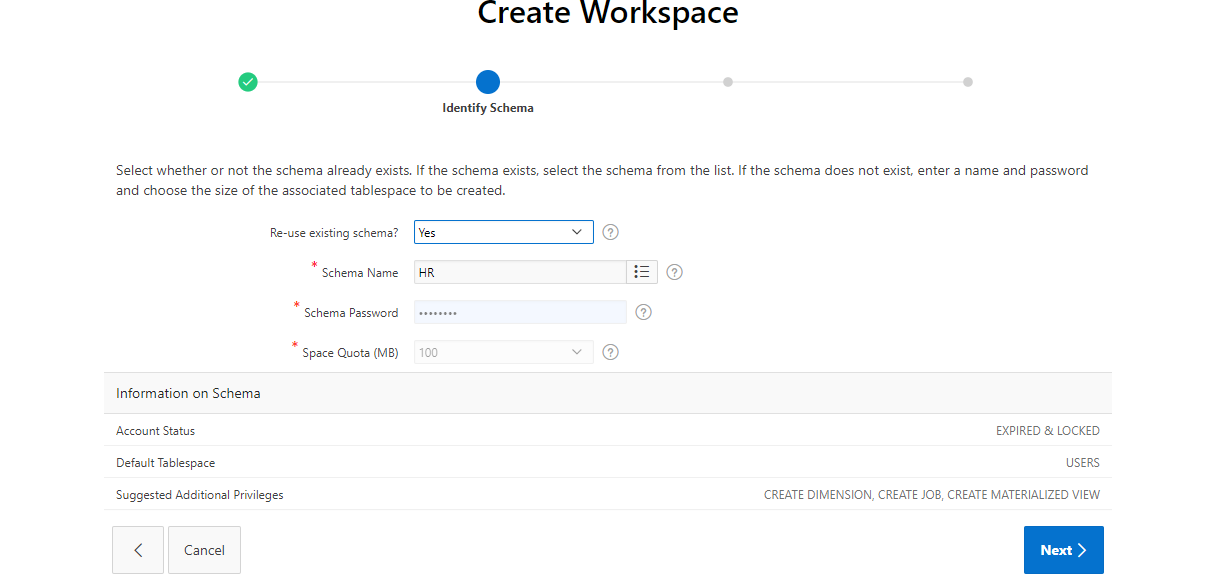
\includegraphics[scale=0.3]{figures/n4.PNG}
        \caption{Pengaturan Pada Skema}
    \end{figure}
    \item Untuk mengubah skema nya menjadi HR, maka klik pada bagian kanan atas ADMIN, nanti akan ada pilihan HR.
    \item Klik next selanjutnya akan muncul tampilan seperti ini.
    \begin{figure}[!htbp]
         \centering
        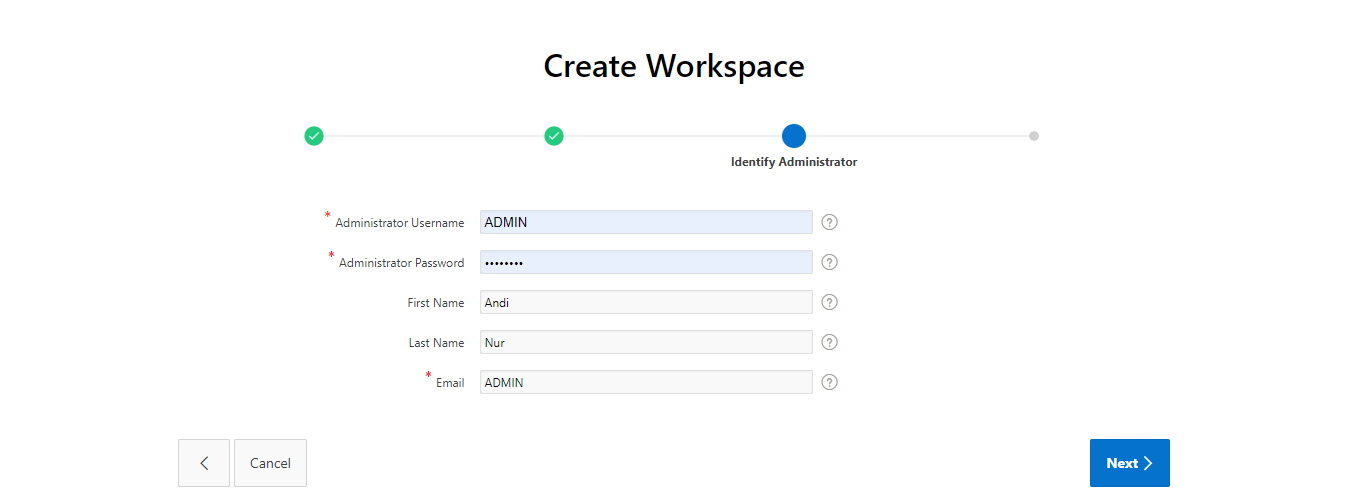
\includegraphics[scale=0.3]{figures/n5.PNG}
        \caption{Pengaturan Administrator}
    \end{figure}
    \item Nantinya, akan mengatur nama username dan password untuk login nantinya.
    \item Setelah itu, atur email dengan email anda. Untuk first dan last name bisa dikosongkan.
     \begin{figure}[!htbp]
        \centering
        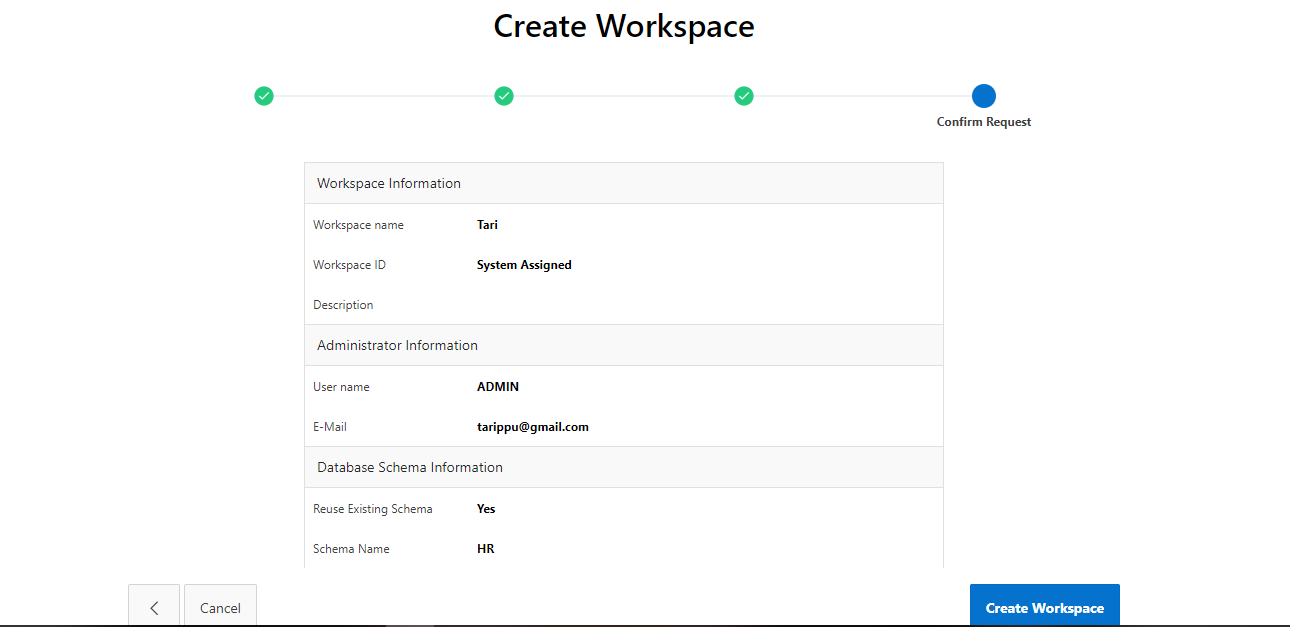
\includegraphics[scale=0.3]{figures/n6.PNG}
        \caption{Login Workspace}
    \end{figure}
    \item Klik next
    \item Setelah next, akan ada konfirmasi kembali mengenai workspace.
    \begin{figure}[!htbp]
        \centering
        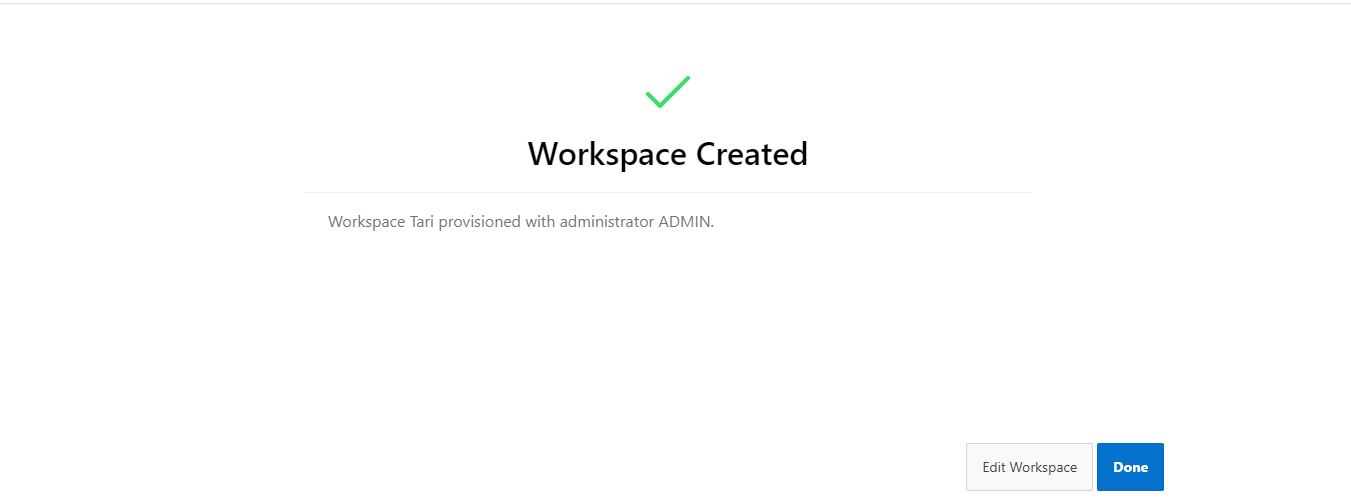
\includegraphics[scale=0.3]{figures/n7.PNG}
        \caption{Konfirmasi Workspace}
    \end{figure}
    \item Jika sudah maka klik create workspace
\newpage
    \item Jika sudah berhasil, maka selanjutnya pergi ke http://127.0.0.1:8080/apex/f?p=4550:10:12402439164670:::::
    \item Maka Login sesuai dengan nama workspace dan username password anda.
    \begin{figure}[!htbp]
        \centering
        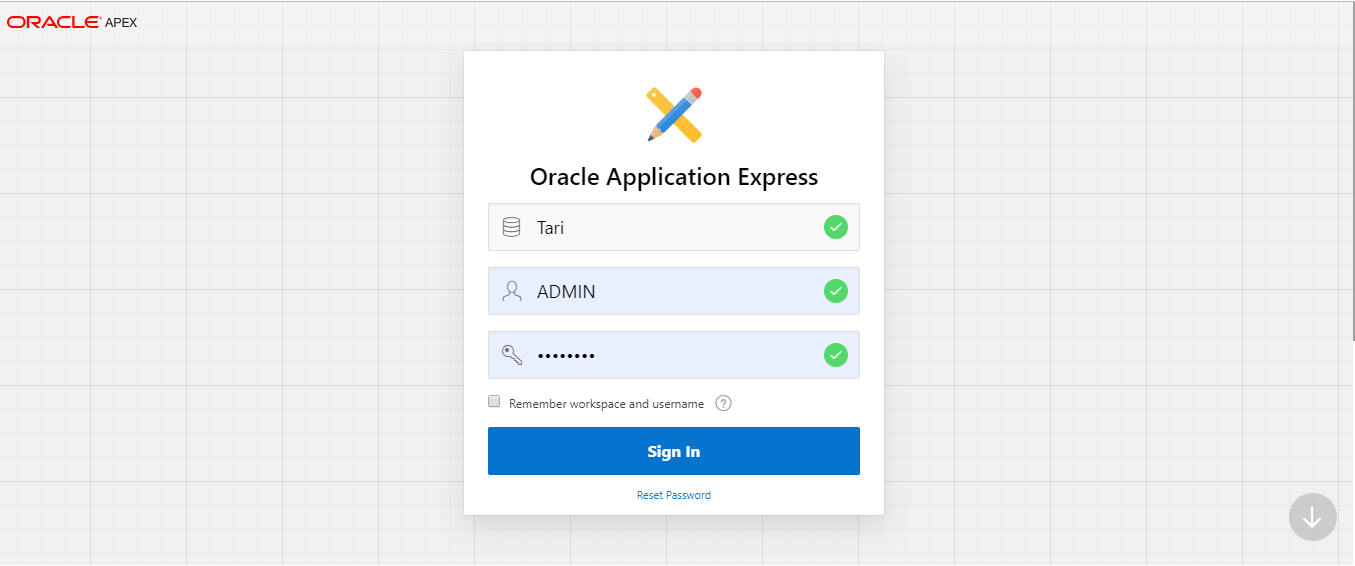
\includegraphics[scale=0.3]{figures/n8.PNG}
        \caption{Atur email dan name Workspace}
    \end{figure}
    \item Setelah login, maka akan ada disuruh ubah password.
    \begin{figure}[!htbp]
        \centering
        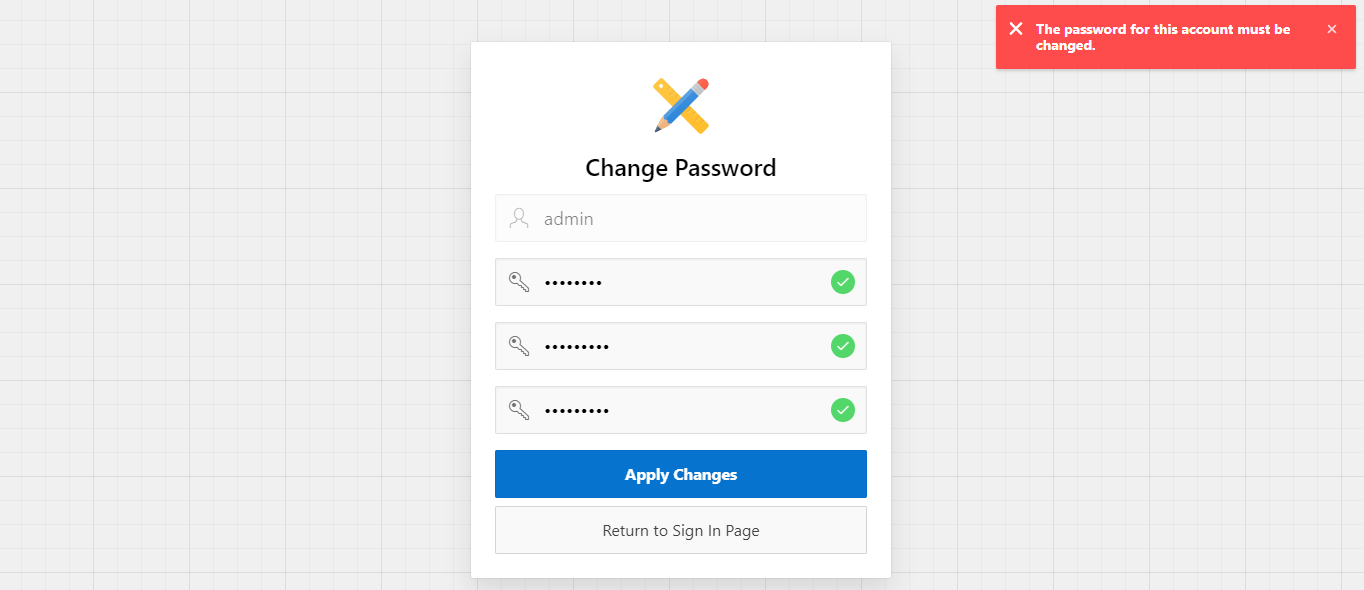
\includegraphics[scale=0.3]{figures/n9.PNG}
        \caption{Hal Ubah Password}
    \end{figure}
\newpage
    \item Akan langsung masuk ke Halaman utama workspace
    \begin{figure}[!htbp]
        \centering
        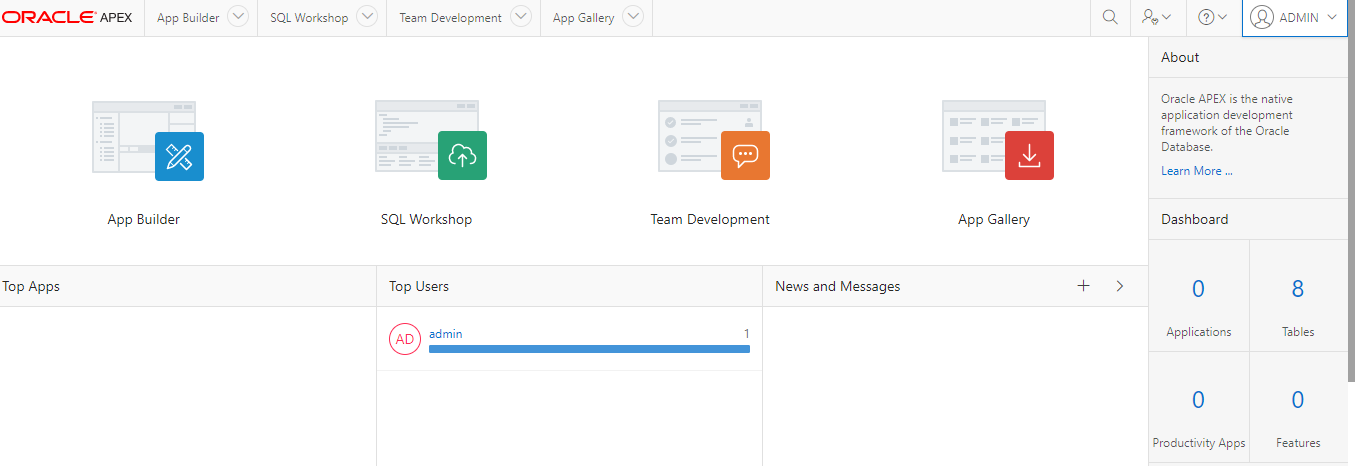
\includegraphics[scale=0.4]{figures/wor1.PNG}
        \caption{Halaman Workspace}
    \end{figure}
\end{enumerate}
\section{Membuat aplikasi pada Oracle Apex}
\begin{enumerate}
    \item Setelah masuk ke halaman workspace, lalu klik App builder
      \begin{figure}[!htbp]
        \centering
        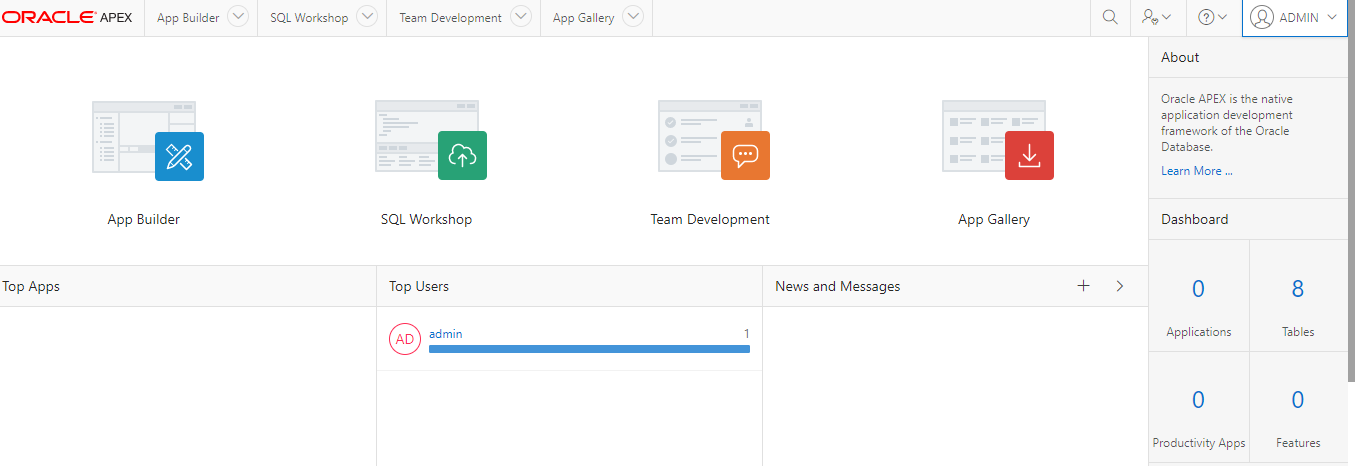
\includegraphics[scale=0.4]{figures/wor1.PNG}
        \caption{Halaman Workspace}
    \end{figure}
    \newpage
         \item Setelah itu klik create
      \begin{figure}[!htbp]
        \centering
        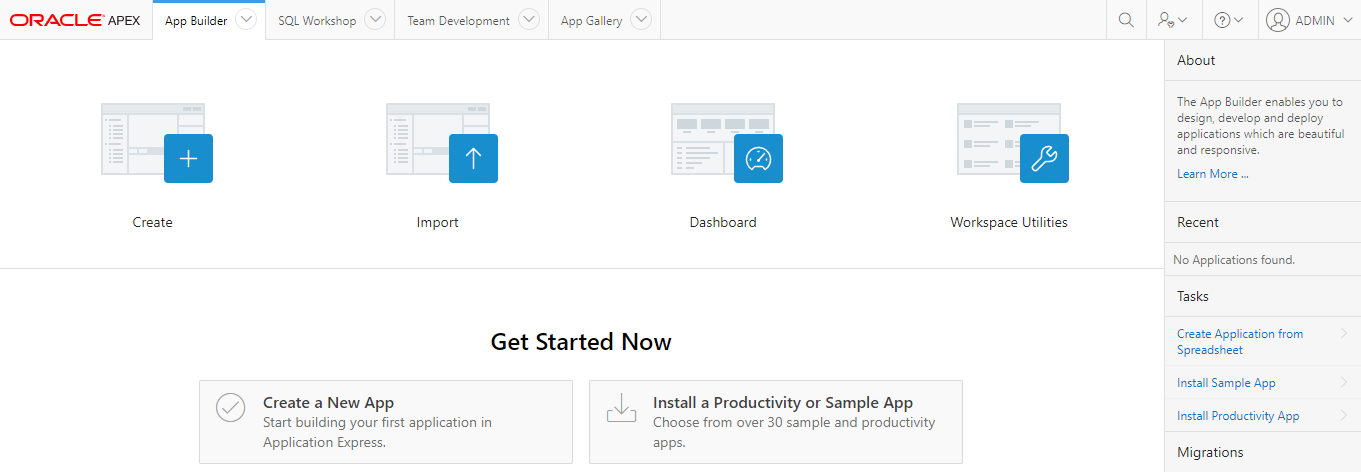
\includegraphics[scale=0.4]{figures/create.PNG}
        \caption{klik create}
    \end{figure}
    \item  pilih new applitaction
      \begin{figure}[!htbp]
        \centering
        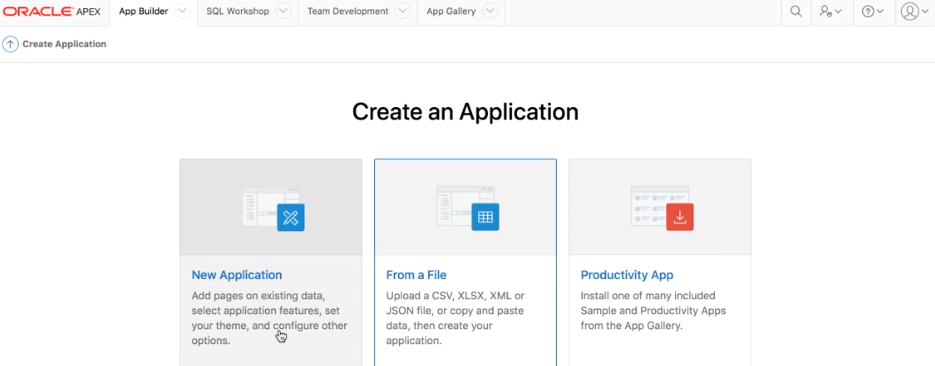
\includegraphics[scale=0.4]{figures/cara2.PNG}
        \caption{New application}
    \end{figure}
    \item Klik check all
      \begin{figure}[!htbp]
        \centering
        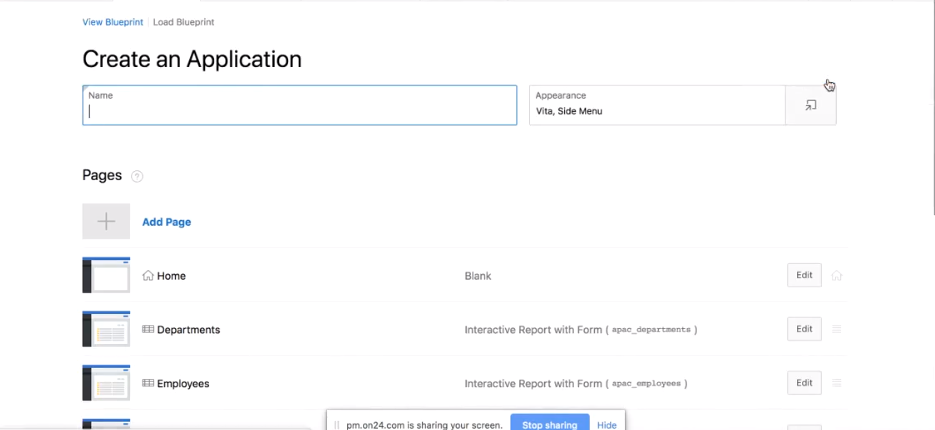
\includegraphics[scale=0.4]{figures/cara7.PNG}
        \caption{Klik check all}
    \end{figure}
    \item Lakukan create aplication
      \begin{figure}[!htbp]
        \centering
        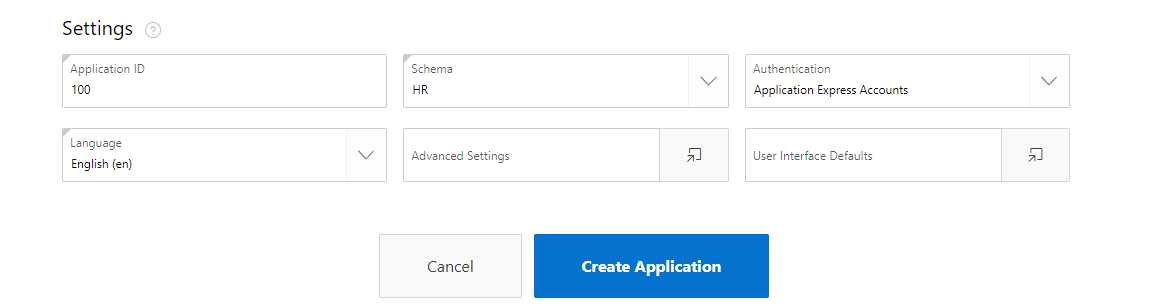
\includegraphics[scale=0.4]{figures/creatapp.PNG}
        \caption{Create application}
    \end{figure}
    \item Tunggu hingga proses create application selesai
    \item Setelah selsai klik run application
      \begin{figure}[!htbp]
        \centering
        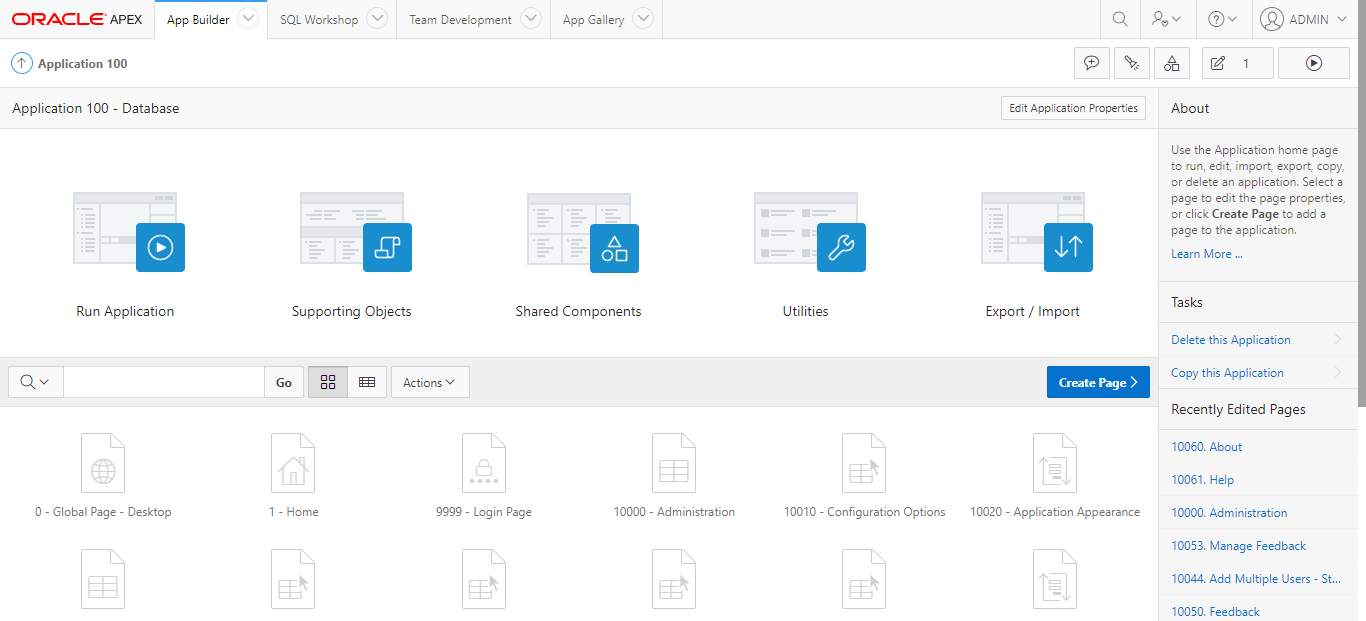
\includegraphics[scale=0.4]{figures/run.PNG}
        \caption{proses creat application}
    \end{figure}
    \item Lalu akan ditampilkan app from spreadsheet
      \begin{figure}[!htbp]
        \centering
        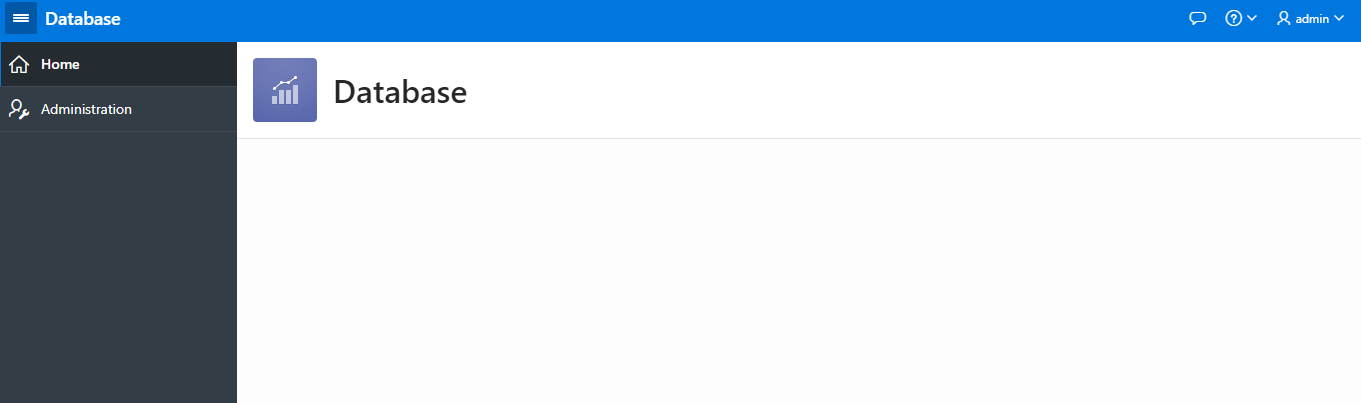
\includegraphics[scale=0.4]{figures/fini.PNG}
        \caption{tampilan app from spreadsheet}
    \end{figure}
\end{enumerate}

